\partepigraph{``Now go out and gather some data, and see what it can do.''}{%
Alon Halevy, Peter Norvig, and Fernando Pereira, \textit{The Unreasonable
Effectiveness of Data}}

\begin{reviewread}
Because clinical text is private, a public model must learn from other biomedical
sources. This part constructs a French biomedical corpus, describes its contents
down to individual paragraphs, and tests which measures of text quality improve
the resulting models.
\end{reviewread}

\chapter{Collecting Biomedical Text}
\label{chap:collecting}
% This chapter is based on the corpus contribution of:
%   Rian Touchent, Laurent Romary, Éric de la Clergerie.
%   CamemBERT-bio: Leveraging Continual Pre-training for
%   Cost-Effective Models on French Biomedical Data.
%   LREC-COLING, 2024.
%
% Pretraining and evaluation: \Cref{chap:encoders}.

\section{Introduction}

Hospitals produce millions of clinical documents every year. These can be used to train language models internally, but the resulting models inherit the legal constraints of their training data: they cannot be released publicly or exchanged between institutions. For a model that is truly open, the training data must come from somewhere else.

Yet hospital records remain the richest source of medical information. Clinical data warehouses have made them increasingly accessible for research purposes. It is estimated that up to 80\% of entities are missing from structured modalities~\citep{raghavan_how_2014}, making clinical reports the richest source of medical information. Yet extracting this information requires high-performing language models adapted to the biomedical domain.

BERT-based models~\citep{devlin_bert_2019} consistently demonstrate state-of-the-art results for a wide range of natural language processing tasks. The adaptation of BERT to the French language, particularly with the CamemBERT model~\citep{martin-etal-2020-camembert}, has replicated these performances in French natural language processing. However, the results of this model on biomedical data are disappointing~\citep{cardon_presentation_2020}, as it exhibits lower performance compared to heuristic models on certain evaluation datasets. These results are predictable because CamemBERT is trained on plain language, often sourced from web pages such as forums. Biomedical data, especially clinical data, are significantly different. They contain technical terms that are very rare or absent in everyday language, and they have a radically distinct style, often telegraphic, rarely consisting of complete sentences, with varying abbreviations.

In this chapter, we address this gap by introducing \textit{biomed-fr}, a public French biomedical corpus of 413 million words assembled from three complementary sources. We describe the corpus construction, analyze the vocabulary mismatch between general and biomedical French tokenizers, and situate our effort among existing French biomedical corpora. The use of this corpus for continual pretraining of CamemBERT, yielding CamemBERT-bio, is presented in \Cref{chap:encoders}.


\section{Existing French Biomedical Corpora}

Several works have attempted to adapt CamemBERT to the biomedical domain, each relying on different training data. \Cref{tab:existing-corpora} summarizes these corpora.

\begin{table}[t]
\centering
\small
\begin{tabular}{llrl}
\toprule
\textbf{Authors} & \textbf{Source} & \textbf{Size} & \textbf{Public} \\
\midrule
\citet{copara_contextualized_2020} & PubMed & 31K docs & Yes \\
\citet{le_clercq_de_lannoy_strategies_2022} & Misc. & 136M words & Partial \\
\citet{dura_learning_2022} & APHP CDW & 21M docs & No \\
\citet{labrak2023drbert} & Misc. & 7.4\,GB & Partial \\
\bottomrule
\end{tabular}
\caption{French biomedical corpora used for language model adaptation. Size units vary across works as reported by their respective authors.}
\label{tab:existing-corpora}
\end{table}

\citet{copara_contextualized_2020} explored a second phase of pre-training on 31,000 French biomedical scientific articles. However, they did not observe a significant improvement on a clinical named entity recognition task using the large version of CamemBERT. This could be explained by the combination of a relatively small corpus (31K documents compared to the 18 billion words in BioBERT) and the large version of the CamemBERT model.

\citet{le_clercq_de_lannoy_strategies_2022} also adapted CamemBERT to the biomedical domain. They aggregated documents from various sources, including PubMed, Cochrane, ISTEX, and Wikipedia, forming a larger partially public corpus of approximately 136 million words. They observed a 2-point improvement in F-measure on a named entity recognition evaluation set composed of drug notices (EMEA), but no significant improvement on a set composed of scientific article titles (MEDLINE).

\citet{dura_learning_2022} continued the pre-training of CamemBERT on 21 million clinical documents from the APHP (Assistance Publique -- Hôpitaux de Paris) clinical data warehouse. They observed a significant 3\% improvement on APMed, a private clinical named entity recognition dataset owned by APHP. They also achieved similar scores to CamemBERT on EMEA and MEDLINE. Their new model performs better on clinical data, yet it obtains scores similar to CamemBERT in other biomedical domains.

\citet{labrak2023drbert} introduced a public French biomedical model named DrBERT. Through their experiments, they explored both continual-pretraining and from-scratch training strategies. Their findings indicated a superior performance when training from scratch, suggesting that continual-pretraining with CamemBERT for French biomedical data may not be as effective. However, when applied to PubMedBERT, continual-pretraining yielded results nearly on par with the from-scratch approach.

Finally, \citet{berhe:hal-03911564} introduced AliBERT, which was trained on a French biomedical corpus primarily comprising articles from ScienceDirect and theses collected through Sudoc. The model leverages a new regularized Unigram-based tokenizer and underwent extensive training on 48 GPUs for a total duration of 20 hours. Their pretrained model outperforms notable French non-domain-specific models, such as CamemBERT and FlauBERT, in two biomedical downstream tasks. Unfortunately, the model is not currently available.


\section{The biomed-fr Corpus}
\label{sec:biomed-fr}

We built a French biomedical corpus composed exclusively of public documents to minimize the usage constraints mentioned earlier. The documents come from three different sources (see \Cref{tab:biomed-fr-composition}), the main one being ISTEX. This new corpus, named \textit{biomed-fr}, consists of 413 million words, equivalent to 2.7\,GB of data. \citet{martin-etal-2020-camembert} have shown that with only 4\,GB of data, it is possible to achieve performance almost comparable to the model trained with the 138\,GB OSCAR dataset~\citep{OrtizSuarezSagotRomary2019}. For an adaptation of CamemBERT to the biomedical domain, this amount of data can be considered sufficient.

\begin{table}[t]
\centering
\small
\begin{tabular}{l S[table-format=3] l}
\toprule
\textbf{Source} & {\textbf{Size (M words)}} & \textbf{Content} \\
\midrule
ISTEX & 276 & Scientific articles \\
CLEAR & 73 & Drug leaflets \\
E3C   & 64 & Clinical cases, leaflets \\
\midrule
\textbf{Total} & \textbf{413} & \\
\bottomrule
\end{tabular}
\caption{Composition of the \textit{biomed-fr} corpus (in millions of words).}
\label{tab:biomed-fr-composition}
\end{table}

\paragraph{ISTEX.} The ISTEX database contains references to 27 million scientific publications. We extracted 108,183 French documents published in a biology or medical journal since 1990. Articles published before this date often contain numerous typographical errors, as they are often scanned articles that require optical character recognition algorithms, resulting in a certain number of errors. Such errors are found to a lesser extent in articles published after 1990. Some documents, although in French, contain passages in English. Therefore, there is an indeterminate amount of English in this corpus. However, it is unlikely that this will significantly impact pre-training. Typographical errors and the presence of other languages are aspects that can be addressed in future versions of \textit{biomed-fr}.

\paragraph{CLEAR.} The CLEAR corpus~\citep{grabar_clear_2018} consists of encyclopedia articles, drug leaflets, and abstracts of scientific articles. Each document is available in two versions: one in technical language and the other in simplified language. We retrieved all of these documents in both versions. Regarding the drug leaflets, we removed redundant sentences at the beginning and end of each document, such as the website navigation bar from which the documents were extracted or information about the company selling the documents.

\paragraph{E3C.} This corpus~\citep{magnini_e3c_2021} is composed of three layers. The first two layers are annotated or semi-annotated and will be used for evaluation in \Cref{chap:encoders}. The last layer is not annotated, and that is the one we retrieved for \textit{biomed-fr}. It consists of medical specialty admission competitions, drug leaflets, and medical thesis abstracts. There may be duplicates of some leaflets found in the CLEAR corpus.

\paragraph{biomed-fr-small.} By randomly selecting 10\% of content from \textit{biomed-fr}, we created a smaller corpus called \textit{biomed-fr-small}. This subset allows us to study the impact of corpus size on downstream performance. Results of this comparison are presented in \Cref{chap:encoders}.


\section{Vocabulary Analysis}
\label{sec:vocab-analysis}

CamemBERT-bio is a biomedical-adapted model based on CamemBERT. Unlike a new model trained from scratch, it shares the same vocabulary. The vocabulary of CamemBERT was constructed using SentencePiece~\citep{kudo_sentencepiece_2018} on an OSCAR sample. Therefore, it is a general-purpose vocabulary designed for everyday language. We can hypothesize that the tokenization of CamemBERT may result in oversplitting of biomedical technical terms.

To investigate this possibility, we trained a specialized tokenizer on \textit{biomed-fr-small} and calculated the intersection of the two vocabularies.

\begin{table}[t]
\centering
\small
\begin{tabular}{lll}
\toprule
\textbf{Term} & \textbf{General} & \textbf{Specialized} \\
\midrule
échocardiographie & écho-cardi-ographie & échocardiographi-e \\
transthoracique   & trans-thorac-ique    & trans-thoracique \\
glimépiride       & g-lim-épi-ride       & gli-m-épi-ride \\
cardiopathie      & cardio-pathie        & cardiopathie \\
diastoliques      & dia-s-tol-iques      & diastolique-s \\
\bottomrule
\end{tabular}
\caption{Comparison of tokenization between a general-purpose tokenizer and a specialized tokenizer for some biomedical technical terms. Hyphens indicate subword boundaries.}
\label{tab:tokenization}
\end{table}

We find a 45\% intersection between the two vocabularies (\Cref{tab:tokenization}), which is quite close to the 42\% intersection found by \citet{beltagy_scibert_2019} between the vocabulary of BERT and SciBERT. Therefore, there is a significant difference in the most frequent terms.

The relatively modest performance gain of PubMedBERT compared to BioBERT and the similar performance of DrBERT compared to CamemBERT-bio despite their specialized vocabulary, together with the over-segmentation of technical terms and the low intersection rate, demonstrate the value of investigating vocabulary adaptation. However, taking into account the comparable performance levels and the significant difference in computational cost (see \Cref{chap:encoders}), we advocate for the continual-pretraining method as the preferred adaptation approach.


\section{Limitations}

It is important to discuss some limitations of our corpus.

Firstly, \textit{biomed-fr} is limited in its diversity. This is because we chose to only use publicly available materials, which tend to lean towards scientific content. As a result, models trained on this corpus may not fully represent performances on real private clinical data. The gap between scientific and clinical text is a recurring challenge that we address in \Cref{chap:content-types}.

Furthermore, we did not explore any potential biases in our data and some parts of the dataset would benefit from further cleaning. These aspects could impact the outputs of models trained on this corpus and should be investigated.

Third, all documents from the selected sources were included indiscriminately, without assessing whether individual passages were genuinely useful for pretraining. Whether such filtering would improve downstream performance is an open question that we explore in \Cref{chap:quality,chap:content-types}.


\section*{Conclusion}

More than half of the most frequent biomedical subwords are absent from CamemBERT's general vocabulary. A mismatch this large raises a natural question: should we abandon the general tokenizer entirely and train a new model from scratch? The answer, perhaps surprisingly, is no, as we show in \Cref{chap:encoders}.

\vspace{2em}

Before we get there, however, a more immediate question deserves attention. We included all 413 million words of \textit{biomed-fr} without filtering. Not all of this text is equally useful. In the next chapter, we investigate whether selecting data by quality can improve upon including everything indiscriminately.


\chapter{Detecting Content Types}
\label{chap:quality}
% This chapter is based on two publications:
%
%   Rian Touchent, Nathan Godey, Éric de la Clergerie.
%   Biomed-Enriched: Data-Efficient Biomedical Pretraining
%   via Paragraph-Level Annotation. ACL, 2026. (first author)
%
%   Nathan Godey*, Wissam Antoun*, Rian Touchent, et al.
%   GAPeron. ACL, 2026. (third author, BiaHS contribution)

\section{Introduction}

For web data, the question of what to keep and what to discard has a straightforward answer. FineWeb-Edu~\citep{penedo2024fineweb} showed that filtering entire documents by educational quality, discarding 92\% of the data, actually improves downstream performance. A low-quality web page is low-quality throughout: if the source is bad, every paragraph is bad. But a scientific article is not a web page.

\begin{figure}[t]
\centering
\begin{tikzpicture}[scale=0.92, transform shape,
  card/.style={rectangle, rounded corners=3pt, line width=0.6pt, text width=4.2cm, align=left, inner sep=6pt, font=\scriptsize\sffamily},
  keepcard/.style={card, fill=ThesisSecondary!30, draw=ThesisSecondaryDark},
  dropcard/.style={card, fill=ThesisTertiary!40, draw=ThesisTertiaryDark},
  arrow/.style={-{Stealth[length=2mm]}, line width=0.8pt, ThesisNeutral}
]

% === LEFT SIDE: Web Document ===
\node[font=\sffamily\small\bfseries, text=ThesisInk] (webtitle) at (-1.7, 0) {Web Document};
\node[font=\sffamily\scriptsize, text=ThesisNeutral, below=1pt of webtitle] (websub) {FineWeb-Edu};

\node[dropcard, below=6pt of websub, minimum height=5.8cm] (web) {
{\tiny\textbf{quality: 2.6}}\\[3pt]
\textit{Session 40 - The Interstellar Medium. Display session, Tuesday}\\[3pt]
Gamma Ray Burst explosions can make kpc-size shells and holes in the ISM of spiral galaxies if much of the energy heats the local gas...\\[3pt]
\textit{Program listing for Tuesday}\\[3pt]
\textit{Previous | Next session}\\[3pt]
\textit{AAS 191st Meeting, January 1998}\\[3pt]
\textit{Session 40 Oral Presentations}
};

\node[font=\sffamily\scriptsize, text=ThesisTertiaryDark, below=6pt of web] {\textbf{Discard entire document}};

% === RIGHT SIDE: PMC Article ===
\node[font=\sffamily\small\bfseries, text=ThesisInk] (pmctitle) at (3.5, 0) {PMC Article};
\node[font=\sffamily\scriptsize, text=ThesisNeutral, below=1pt of pmctitle] (pmcsub) {Biomed-Enriched (ours)};

% P1: review
\node[keepcard, below=6pt of pmcsub] (p1) {
{\tiny\textbf{quality: 4.8}\hfill\textbf{type: review}}\\[2pt]
Pulmonary hypertension is a progressive cardiopulmonary disorder characterized by elevated pulmonary arterial pressure.
};

% P2: other
\node[dropcard, below=8pt of p1] (p2) {
{\tiny\textbf{quality: 1.4}\hfill\textbf{type: other}}\\[2pt]
Based on this preliminary work, we developed an initial draft document shared with the group for revision.
};

% P3: case
\node[keepcard, below=8pt of p2] (p3) {
{\tiny\textbf{quality: 4.3}\hfill\textbf{type: case}}\\[2pt]
A 27-year-old female presented with four episodes of exertional syncope. Catheterization revealed mPAP 43 mmHg.
};

% Frame around PMC paragraphs
\begin{scope}[on background layer]
\node[fit=(p1)(p2)(p3), fill=ThesisPaper, draw=ThesisNeutral!40, rounded corners=4pt, inner sep=5pt] {};
\end{scope}

% Arrows
\draw[arrow, ThesisSecondaryDark] (p1.east) -- ++(0.3, 0) node[right, font=\sffamily\tiny, text=ThesisSecondaryDark] {keep};
\draw[arrow, ThesisTertiaryDark] (p2.east) -- ++(0.3, 0) node[right, font=\sffamily\tiny, text=ThesisTertiaryDark] {filter};
\draw[arrow, ThesisSecondaryDark] (p3.east) -- ++(0.3, 0) node[right, font=\sffamily\tiny, text=ThesisSecondaryDark] {keep};

\end{tikzpicture}
\caption{\textbf{Document-level vs.\ paragraph-level filtering.} A low-quality web page can be discarded entirely (left). A scientific article mixes high-value content (clinical cases, reviews) with boilerplate (right). Paragraph-level annotation allows keeping the valuable parts.}
\label{fig:motivation}
\end{figure}
% TODO: replace example paragraphs with real extracts from a single PMC article

\Cref{fig:motivation} illustrates the difference. A web page about astronomy scores low throughout and can be safely discarded. A PMC article on pulmonary hypertension, by contrast, contains a textbook-quality review paragraph, a boilerplate committee note, and a clinical case report with real diagnostic values. Document-level filtering would either keep all three or discard all three. Neither is the right answer.

In the previous chapter, we assembled \textit{biomed-fr} by including all available documents from three public sources. This approach treats every paragraph equally. How much of this text actually helps, what types of content does it contain, and can we be smarter about what we include?

In this chapter, we introduce a paragraph-level annotation framework that distinguishes content types, domains, and educational quality within scientific articles. We show that selective pretraining on the most relevant paragraphs matches the performance of training on the full corpus using one-third of the tokens. We also extract 2 million clinical case paragraphs from PubMed Central, providing an openly available alternative to restricted hospital records. Finally, we investigate the risks of neural quality filtering: not all selection strategies are equally safe, and some can amplify benchmark contamination by a factor of 20.


\section{Content Heterogeneity in Scientific Articles}
\label{sec:heterogeneity}

% === EXAMPLE: mixed content in a single article ===
% TODO: Add a concrete example here — a real PMC article showing
% a clinical case paragraph, a methods paragraph, and a boilerplate
% paragraph side by side, with their annotation scores.

Large language models for biomedicine are typically pretrained on PubMed Central (PMC) Open Access articles. While valuable, this corpus presents challenges including heterogeneous quality, predominance of English content (approximately 98\%), uneven representation of clinical cases, and variable educational value. Existing filtering approaches operate at the article level: BioMistral~\citep{labrak-etal-2024-biomistral} upsampled non-English articles, while Meditron~\citep{chen2023meditron} scored articles using MeSH tags, publication type, journal reputation, recency, and citation count. These methods assume that entire documents are either valuable or not.

This assumption does not hold for curated scientific corpora. Unlike web-scraped data where low-quality sources justify discarding entire documents, scientific articles are all potentially valuable. The real issue is variance \emph{within} articles. To quantify this, we analyzed 10,000 PMC articles (378,000 paragraphs) and found that 91.6\% of articles contain multiple document types (clinical case, study, review, other). Educational scores vary by 2.6 points on average within articles, spanning more than half of the 1--5 scale. Some paragraphs contain excellent educational or clinical content, while others add little domain knowledge but remain difficult to detect with simple heuristics.

\begin{table}[t]
\centering
\small
\begin{tabular}{lrr}
\toprule
& \textbf{Single} & \textbf{Mixed} \\
\midrule
Document Type & 8.4\% & 91.6\% \\
Domain & 44.7\% & 55.3\% \\
\midrule
\multicolumn{3}{l}{\textit{Educational Score (1--5 scale)}} \\
\midrule
& \textbf{Mean} & \textbf{Median} \\
Intra-article std & 0.68 & 0.70 \\
Intra-article range & 2.61 & 2.86 \\
\bottomrule
\end{tabular}
\caption{Intra-document heterogeneity in 10K PMC articles (378K paragraphs). 91.6\% of articles contain multiple document types. Educational scores vary by 2.6 points on average within articles.}
\label{tab:heterogeneity}
\end{table}


\section{Method}

\subsection{Data Collection and Preprocessing}
\label{sec:data-collection}

We extracted text from the PubMed Central (PMC) Open Access Subset, containing approximately 4.5 million full-text scientific articles. Using a custom pipeline, we processed the raw XML files to extract article content, segment articles into 133 million individual paragraphs, filter out non-textual elements, and retain only paragraphs containing a minimum of 64 tokens.

\subsection{Two-Stage Annotation Framework}
\label{sec:annotation}

We follow a two-stage annotation process on a single 8$\times$A100 node: 160 GPU-hours for the first stage and 80 GPU-hours for the second.

\paragraph{Stage 1: LLM annotation.}
We used Llama-3.1-70B-Instruct~\citep{touvron2024llama3} to annotate a diverse subset of 400,000 paragraphs (approximately 0.33\% of the corpus) across multiple dimensions: type classification (clinical case, study, review, other), domain categorization (clinical, biomedical, other), and educational quality (1--5 scale). Language was identified separately using langdetect.

% TODO: include annotation prompt in appendix, reference it here

\paragraph{Stage 2: Distillation.}
To scale annotation to the full corpus, we distilled the LLM annotations into a smaller XLM-RoBERTa-base model~\citep{conneau2020xlmr} trained to jointly predict all annotation dimensions. On 39,800 held-out paragraphs, the student closely matches the Llama-3.1-70B labels (\Cref{tab:distillation}). It is important to note that these annotations are not gold-standard labels verified by medical experts, but neural heuristics for data curation. Similar to FineWeb-Edu~\citep{penedo2024fineweb}, they guide which content to prioritize during pretraining.

\begin{table}[t]
\centering
\small
\begin{tabular}{lc}
\toprule
\textbf{Dimension} & \textbf{Agreement} \\
\midrule
Educational score & $r = 0.876$, MAE $= 0.326$ \\
Domain & $F_1 = 0.954$ \\
Document type & $F_1 = 0.925$, $\kappa = 0.821$ \\
\bottomrule
\end{tabular}
\caption{Distillation quality: agreement between the XLM-RoBERTa student and Llama-3.1-70B teacher on held-out paragraphs.}
\label{tab:distillation}
\end{table}

\begin{figure}[t]
\centering
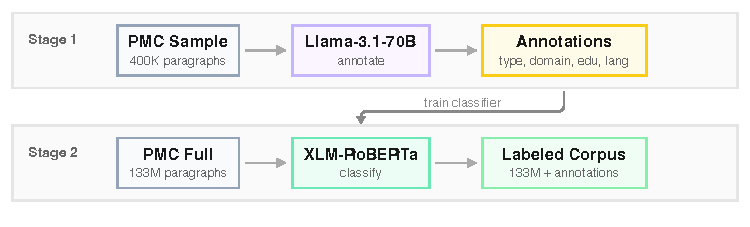
\includegraphics[width=\columnwidth]{sources/part_1/chapter2/imgs/pipeline.pdf}
\caption{\textbf{Two-stage annotation pipeline.} Stage~1: Llama-3.1-70B annotates 0.33\% of PMC paragraphs across four dimensions. Stage~2: a fine-tuned XLM-RoBERTa distills these annotations to label the full corpus, enabling flexible filtering strategies.}
\label{fig:pipeline}
\end{figure}

\subsection{Data Analysis}
\label{sec:data-analysis}

Most PMC paragraphs receive an educational score of 4, with a mean of 3.48 and median of 4.00. This distribution varies by content type: reviews and studies contain the highest proportion of educational content (86.9\% and 78.7\% scoring 4, respectively), while clinical cases show more variance (57.0\% rated 4). Domain-wise, biomedical paragraphs score higher (75.3\% at score 4) than clinical text (44.0\%), and content labeled ``other'' rarely reaches high scores (2.1\%). These patterns support the score threshold ($\geq 3$) used in BE-Educational and BE-All, and explain why combining domain and quality filters yields consistent gains across tasks.

\begin{figure}[t]
\centering
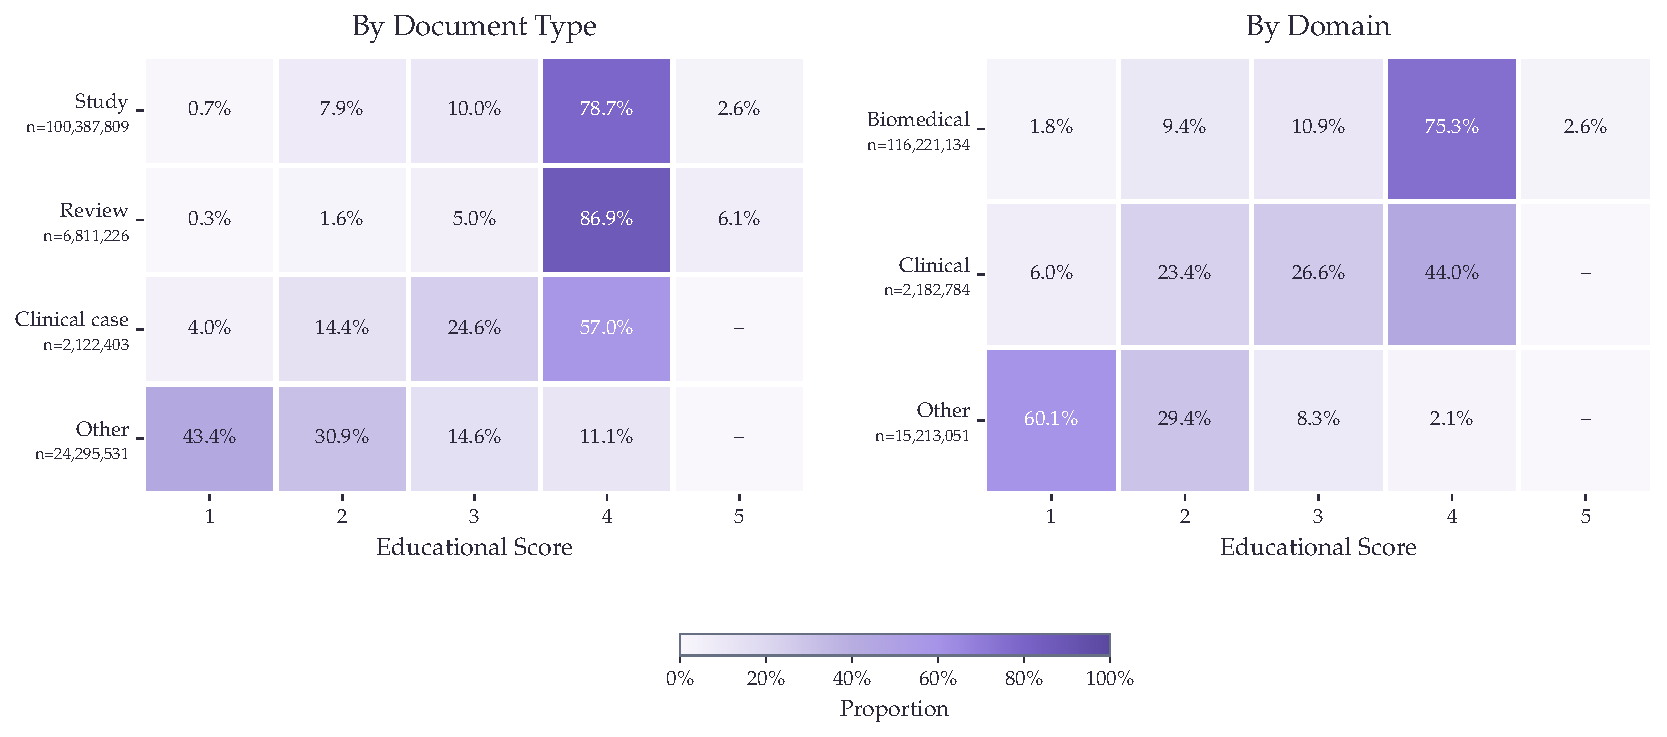
\includegraphics[width=\columnwidth]{plots/chapter2/combined_educational_scores.pdf}
\caption{\textbf{Distribution of educational quality scores by document type and domain.} Reviews and studies show the highest proportion of high scores, while clinical texts display more variance. Content labeled ``other'' rarely reaches high scores.}
\label{fig:edu-scores}
\end{figure}

\subsection{Dataset Construction}
\label{sec:dataset}

Using the distilled model, we annotated the full PMC corpus and constructed several dataset variants through strategic filtering and upsampling, summarized in \Cref{tab:be-variants}. Upsampling refers to duplicating articles in the training corpus, proportionally increasing their sampling probability.

% TODO: add example of a clinical case paragraph extracted from a
% genomics article — showing that clinical content hides in unexpected places

\begin{table}[t]
\centering
\small
\renewcommand{\arraystretch}{1.6}
\begin{tabular}{lp{8.5cm}}
\toprule
\textbf{Variant} & \textbf{Strategy} \\
\midrule
BE-Base & Complete unmodified PMC Open Access Subset (baseline). \\
BE-Educational & Removes paragraphs with educational quality scores below 3. \\
BE-Clinical & Upsamples 10$\times$ articles with predominantly clinical domain content. \\
BE-ClinicalCase & Upsamples 10$\times$ articles containing at least one clinical case paragraph. \\
BE-French & Upsamples 10$\times$ articles containing French text. \\
BE-All & Combines quality filtering (score $\geq 3$), upsampling of clinical content, French text, and clinical cases, plus metadata prefixing. \\
\bottomrule
\end{tabular}
\renewcommand{\arraystretch}{1.0}
\caption{Biomed-Enriched dataset variants. All variants preserve the original article structure and use an 8K context window during pre-training.}
\label{tab:be-variants}
\end{table}

For all variants, we preserved the original structure of the article and employed an 8K context window during pre-training. This ensures that models can process complete scientific articles, capturing dependencies where information presented in earlier paragraphs is essential for understanding later content.


\section{Experimental Setup}
\label{sec:experimental-setup}

Continual pre-training served as a method to evaluate the relevance and utility of our annotations. Our evaluation focuses on isolating the effects of data curation rather than pursuing state-of-the-art scores on benchmarks. A more powerful foundation model would likely yield higher absolute scores, but would probably obscure the precise impact of our dataset.

\subsection{Decoder Setup}

We selected OLMo2-7B-stage1~\citep{olmo2025furious} as our foundation model for continual pre-training, strategically choosing this intermediate checkpoint to more clearly attribute performance changes to our data curation. Although stage~1 has already developed strong language modeling capabilities, it precedes the knowledge-intensive tuning of stage~2, providing an ideal balance of baseline capabilities without the risk of catastrophic forgetting of instruction-following abilities during domain adaptation. Notably, the data mix used in stage~1 includes DCLM~\citep{li2024datacomp}, which is a dataset obtained by filtering web-data using a classifier trained on instruct-data. Hence, OLMo2-7B already has relatively strong question-answering capabilities after stage~1.

Each Biomed-Enriched variant was trained with exactly 33.6 billion tokens, using identical hyperparameters. We follow the annealing strategy of OLMo2 used in the mid-training phase. By maintaining strict parameter parity across experiments, we created a controlled environment focused solely on measuring the effectiveness of our different data curation strategies.

\subsection{Encoder Setup}

We also conducted continual-pretraining experiments on encoder models. Starting from ModernBERT-base~\citep{modernbert} after its context extension phase, we followed exactly the same hyperparameters as BioClinical-ModernBERT phase~1. Our baseline reproduces their standard continual pretraining setup on public PubMed/PMC. Our clinical-upsample recipe additionally applies educational filtering (score $\geq 3$) and upsamples clinical cases 100$\times$ and clinical domain content 10$\times$.

\Cref{tab:hyperparams} summarizes the hyperparameters for both setups.

\begin{table}[t]
\centering
\small
\begin{minipage}[t]{0.48\textwidth}
\centering
\begin{tabular}{ll}
\toprule
\textbf{Parameter} & \textbf{Value} \\
\midrule
Base model & OLMo2-7B-stage1 \\
Peak LR & 6.15e-5 \\
Min LR & 6.15e-6 \\
LR Decay & Linear \\
Batch size & 1024 \\
Weight decay & 0.1 \\
Context & 8,192 tokens \\
Hardware & 128 MI250X \\
Tokens & 33.6B / variant \\
\bottomrule
\end{tabular}
\subcaption{Decoder}
\label{tab:decoder-hyperparams}
\end{minipage}%
\hfill
\begin{minipage}[t]{0.48\textwidth}
\centering
\begin{tabular}{ll}
\toprule
\textbf{Parameter} & \textbf{Value} \\
\midrule
Base model & ModernBERT-base \\
Peak LR & 5e-4 \\
Min LR & 5e-7 \\
LR Decay & one\_minus\_sqrt \\
Batch size & 576 \\
Weight decay & 1e-5 \\
Context & 8,192 tokens \\
Hardware & 4$\times$ H100 \\
Tokens & 70B \\
\bottomrule
\end{tabular}
\subcaption{Encoder}
\label{tab:encoder-hyperparams}
\end{minipage}
\caption{Hyperparameters for continual pre-training.}
\label{tab:hyperparams}
\end{table}

\subsection{Evaluation}

For decoders, our evaluation consists of zero-shot testing on MMLU medical subcategories, MedQA~\citep{jin2021medqa}, MedMCQA~\citep{pal2022medmcqa}, and PubMedQA~\citep{jin2019pubmedqa}. For the French adaptation assessment, we use 5-shot evaluation on FrenchMedMCQA~\citep{labrak-etal-2022}. We compare our models against three baselines: OLMo2-7B-stage1, Llama-3.1-8B, and Meditron-70B.

For the encoder models, we evaluate on 11 tasks spanning clinical and biomedical domains. Clinical tasks include ChemProt, Phenotype, COS, SocialHistory, and DEID. Biomedical tasks include AnatEM, BC5CDR, JNLPBA, NCBI Disease, GAD, and Hallmarks of Cancer. Following the evaluation recipe of BioClinical-ModernBERT, we finetune for 10 epochs on clinical tasks and 20 epochs on biomedical tasks, with early stopping patience of 3 epochs for all. We compare against BioClinical-ModernBERT~\citep{sounack2025bioclinicalmodernbert}, which was trained on 169B tokens from PubMed, PMC, and 20 clinical datasets including MIMIC-III, MIMIC-IV, CheXpert Plus radiology reports, and various clinical notes from multiple institutions, most requiring data use agreements.


\section{Results}
\label{sec:results}

\subsection{Decoder Results}

\Cref{tab:decoder-qa,tab:decoder-mmlu} present decoder results on medical QA and MMLU benchmarks. The combined strategy BE-All achieves the best average performance (61.08\%), with the strongest gains on MedQA (+2.4 pts) and MMLU Clinical Knowledge (+1.5 pts). Different enrichment strategies show complementary strengths: clinical upsampling yields a +4 point improvement on MMLU Professional Medicine, while educational filtering improves Medical Genetics by +2 points and MedMCQA by +1.2 points. BE-All reaches target performance using roughly one-third of the training tokens compared to BE-Base, with stable improvements visible from early checkpoints. BE-French also demonstrates successful adaptation to French medical QA (40.5\% vs 38.3\% baseline, \Cref{fig:french-performance}), showing that language-specific upsampling generalizes beyond English.

\begin{figure}[t]
\centering
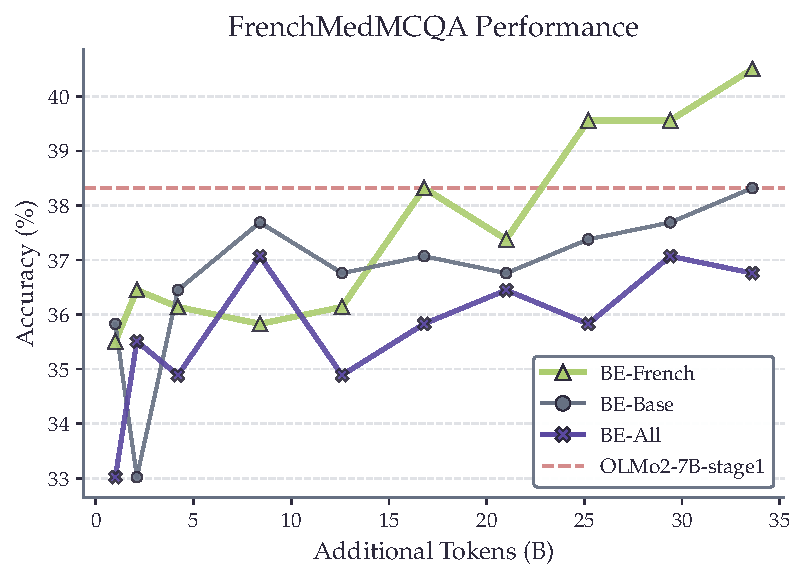
\includegraphics[width=0.55\columnwidth]{plots/chapter2/french_medmcqa_performance.pdf}
\caption{\textbf{FrenchMedMCQA performance.} BE-French outperforms other variants on French medical QA, demonstrating effective language-specific improvement through targeted upsampling.}
\label{fig:french-performance}
\end{figure}

\begin{table}[t]
\centering
\small
\setlength{\tabcolsep}{8pt}
\sisetup{detect-weight=true}
\begin{threeparttable}[b]
\begin{tabular}{l S[table-format=2.2] S[table-format=2.2] S[table-format=2.2] S[table-format=2.2]}
\toprule
\textbf{Model} & {\textbf{MedQA}} & {\textbf{MedMCQA}} & {\textbf{PubMedQA}} & {\textbf{Avg}} \\
\midrule
\rowcolor{ThesisTableSep}
\multicolumn{5}{c}{\rule{0pt}{10pt}\textbf{Reference Models}} \\[1pt]
Llama-3-8B & 59.70 & 57.47 & 74.80 & 63.99 \\
Meditron-70B & 57.10 & 46.80 & 76.60 & 60.17 \\
\midrule
\rowcolor{ThesisTableSep}
\multicolumn{5}{c}{\rule{0pt}{10pt}\textbf{Our Variants}} \\[1pt]
OLMo2-7B-stage1 & 45.33 & 41.14 & 75.60 & 54.02 \\
\quad + BE-Base & 44.85 & 41.91 & 76.40 & 54.39 \\
\quad + BE-Clinical & 41.95 & 39.35 & 76.60 & 52.63 \\
\quad + BE-ClinicalCase & 42.11 & 39.52 & 76.60 & 52.74 \\
\quad + BE-Educational & 45.64 & \bfseries 43.08 & \underline{77.00} & \underline{55.24} \\
\quad + BE-All (33.6B) & \bfseries 47.21 & 42.79 & 76.60 & 55.53 \\
\quad + BE-All (12.6B) & \bfseries 47.21 & \underline{42.94} & 76.40 & \bfseries 55.52 \\
\bottomrule
\end{tabular}
\begin{tablenotes}
  \small
  \item Bold indicates best result per column. Underline: second-best.
\end{tablenotes}
\end{threeparttable}
\caption{\textbf{Decoder results: Medical QA benchmarks.} BE-All achieves the best QA average with both 33.6B and 12.6B tokens.}
\label{tab:decoder-qa}
\end{table}

\begin{table}[t]
\centering
\small
\setlength{\tabcolsep}{6pt}
\sisetup{detect-weight=true}
\begin{threeparttable}[b]
\begin{tabular}{l S[table-format=2.2] S[table-format=2.2] S[table-format=2.2] S[table-format=2.2] S[table-format=2.2] S[table-format=2.2] S[table-format=2.2]}
\toprule
\textbf{Model} & {\textbf{Anat}} & {\textbf{Clin}} & {\textbf{Bio}} & {\textbf{Med}} & {\textbf{Gen}} & {\textbf{Prof}} & {\textbf{Avg}} \\
\midrule
\rowcolor{ThesisTableSep}
\multicolumn{8}{c}{\rule{0pt}{10pt}\textbf{Reference Models}} \\[1pt]
Llama-3-8B & 68.89 & 74.72 & 78.47 & 61.85 & 83.00 & 70.22 & 72.86 \\
Meditron-70B & 53.30 & 66.70 & 76.30 & 63.00 & 69.00 & 71.60 & 66.65 \\
\midrule
\rowcolor{ThesisTableSep}
\multicolumn{8}{c}{\rule{0pt}{10pt}\textbf{Our Variants}} \\[1pt]
OLMo2-7B-stage1 & 54.81 & 63.40 & \underline{69.44} & 53.18 & \underline{69.00} & 59.93 & 61.63 \\
\quad + BE-Base & \underline{57.04} & 64.15 & \bfseries 70.83 & \bfseries 59.54 & \underline{69.00} & 59.93 & 63.42 \\
\quad + BE-Clinical & 53.33 & 63.40 & 65.28 & 58.38 & 66.00 & \bfseries 63.97 & 61.73 \\
\quad + BE-ClinicalCase & 57.04 & 64.91 & 66.67 & \bfseries 59.54 & \underline{69.00} & \underline{62.87} & 63.34 \\
\quad + BE-Educational & 57.04 & \underline{65.28} & 68.06 & 56.65 & \bfseries 71.00 & 58.82 & 62.81 \\
\quad + BE-All (33.6B) & \underline{60.00} & \bfseries 65.66 & 68.06 & \underline{58.96} & \underline{69.00} & 61.40 & \underline{63.85} \\
\quad + BE-All (12.6B) & \bfseries 64.44 & 64.53 & 68.75 & 57.23 & \bfseries 71.00 & \underline{62.87} & \bfseries 64.80 \\
\bottomrule
\end{tabular}
\begin{tablenotes}
  \small
  \item Anat=Anatomy, Clin=Clinical Knowledge, Bio=College Biology, Med=College Medicine, Gen=Medical Genetics, Prof=Professional Medicine.
\end{tablenotes}
\end{threeparttable}
\caption{\textbf{Decoder results: MMLU Medical subcategories.} BE-All (12.6B) achieves the best MMLU average despite using one-third of the tokens.}
\label{tab:decoder-mmlu}
\end{table}

\begin{figure}[t]
\centering
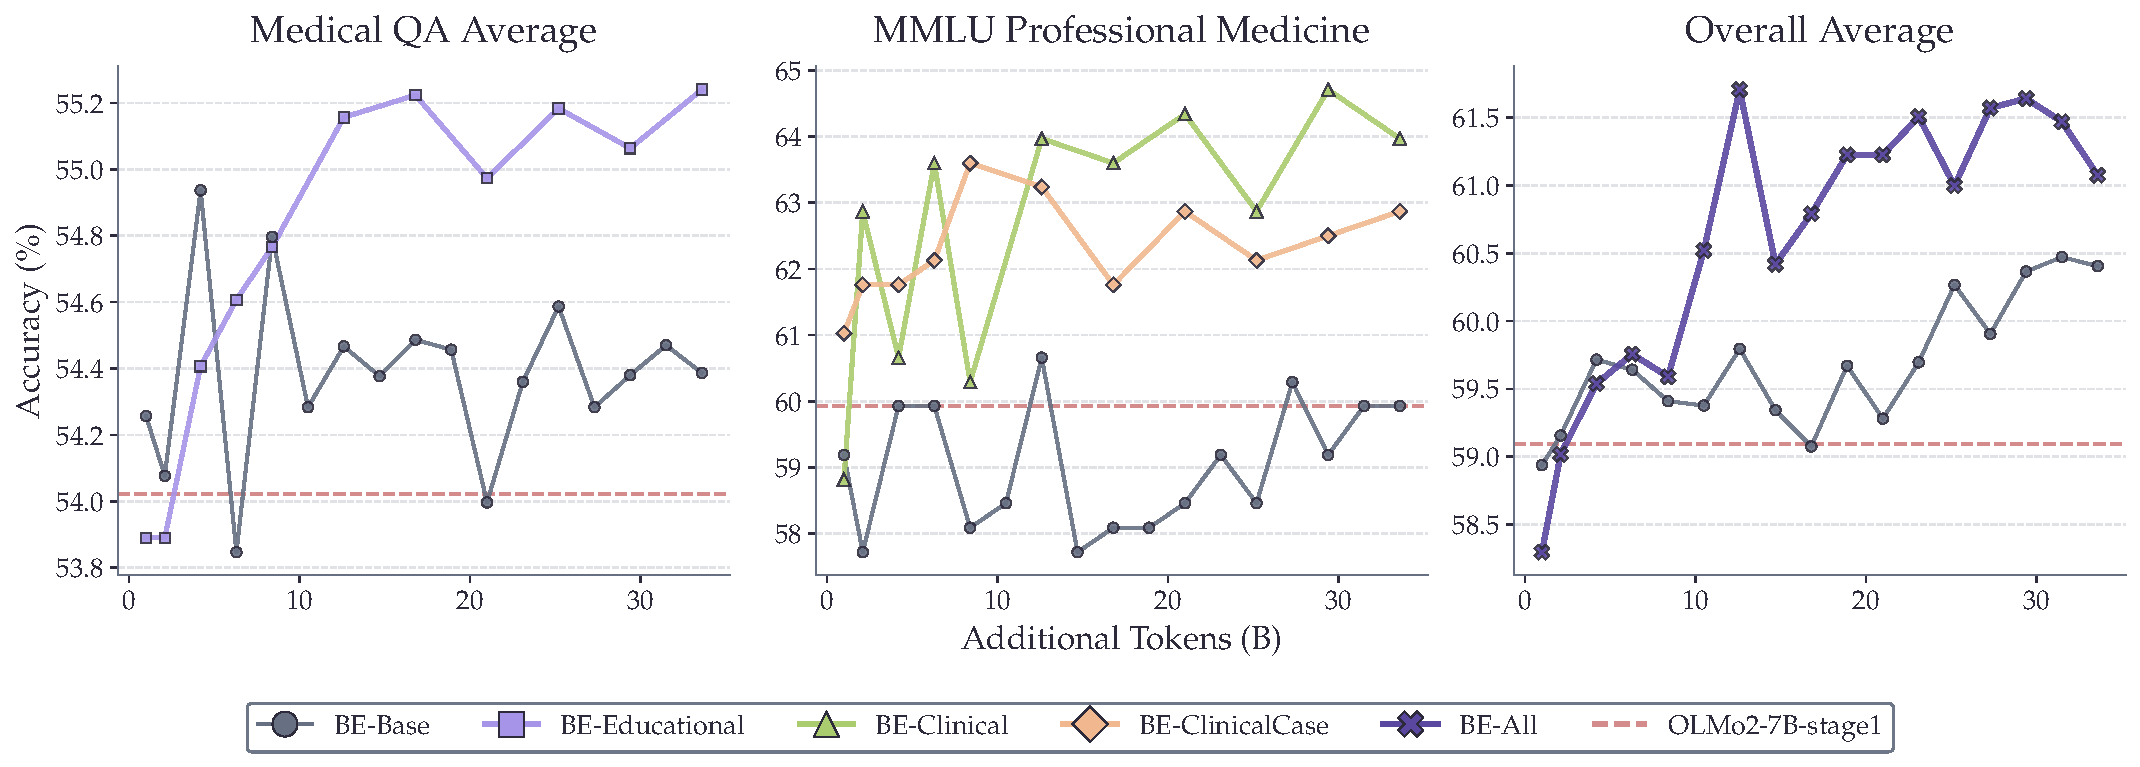
\includegraphics[width=\columnwidth]{plots/chapter2/combined_plot_v2.pdf}
\caption{\textbf{Decoder training progression.} BE-All reaches target performance with approximately one-third of the training tokens required by BE-Base.}
\label{fig:decoder-curves}
\end{figure}

\subsection{Encoder Results}

\Cref{tab:encoder-clinical,tab:encoder-biomed} present encoder results across 11 clinical and biomedical benchmarks. Our BE-Clinical recipe achieves 77.08\% average $F_1$, matching BioClinical-ModernBERT (77.05\%) while using 2.5$\times$ fewer tokens and only public PubMed/PMC data. Adding a decay phase with high-quality educational content brings slight additional gains: the Biomedical decay variant (edu $\geq 4$) achieves 77.32\%.

Different decay targets show task-specific strengths: Study decay yields the best results on AnatEM (79.7\%) and NCBI Disease (81.2\%), Review decay excels on GAD (80.2\%), and Clinical Case decay achieves the highest SocialHistory score (57.0\%). These results suggest that public PMC data has more potential for clinical NLP than commonly exploited, and that targeted curation can close the gap with models trained on restricted datasets.

\begin{table}[t]
\centering
\small
\setlength{\tabcolsep}{6pt}
\sisetup{detect-weight=true}
\begin{threeparttable}[b]
\begin{tabular}{l S[table-format=2.1] S[table-format=2.1] S[table-format=2.1] S[table-format=2.1] S[table-format=2.1] S[table-format=2.1]}
\toprule
\textbf{Model} & {\textbf{ChemPr}} & {\textbf{Pheno}} & {\textbf{COS}} & {\textbf{Social}} & {\textbf{DEID}} & {\textbf{Avg}} \\
\midrule
\rowcolor{ThesisTableSep}
\multicolumn{7}{c}{\rule{0pt}{10pt}\textbf{Baselines}} \\[1pt]
ModernBERT-base & 89.5 & 48.4 & 94.0 & 53.1 & 78.3 & 72.66 \\
BioClinical-MdnBERT\tnote{$\dagger$} & 90.0 & \bfseries 60.7 & 94.8 & 56.0 & \bfseries 81.8 & \bfseries 76.66 \\
\midrule
\rowcolor{ThesisTableSep}
\multicolumn{7}{c}{\rule{0pt}{10pt}\textbf{Our Models (Public Data Only)}} \\[1pt]
Baseline & 89.8 & 59.6 & 94.5 & 55.5 & 78.5 & 75.58 \\
BE-Clinical & 89.9 & 59.9 & 94.8 & 56.8 & 79.7 & 76.22 \\
\midrule
\rowcolor{ThesisTableSep}
\multicolumn{7}{c}{\rule{0pt}{10pt}\textbf{With Decay Phase}} \\[1pt]
\quad + Review & \bfseries 90.3 & 59.7 & 94.6 & 55.4 & 79.6 & 75.92 \\
\quad + Study & \bfseries 90.3 & \bfseries 60.3 & 94.7 & 55.6 & 78.6 & 75.90 \\
\quad + Clinical Case & 89.5 & 59.4 & 94.5 & \bfseries 57.0 & 79.3 & 75.94 \\
\quad + Biomedical & 90.1 & 59.9 & \bfseries 94.9 & 56.4 & 79.6 & \underline{76.18} \\
\bottomrule
\end{tabular}
\begin{tablenotes}
  \small
  \item[$\dagger$] Trained on 169B tokens including 20 clinical datasets (MIMIC-III/IV, CheXpert, etc.). Our models use only public PubMed/PMC.
  \item ChemPr=ChemProt, Pheno=Phenotype, Social=SocialHistory.
\end{tablenotes}
\end{threeparttable}
\caption{\textbf{Encoder results: Clinical tasks.} Our BE-Clinical recipe matches BioClinical-ModernBERT on clinical tasks using only public data.}
\label{tab:encoder-clinical}
\end{table}

\begin{table}[t]
\centering
\small
\setlength{\tabcolsep}{5pt}
\sisetup{detect-weight=true}
\begin{threeparttable}[b]
\begin{tabular}{l S[table-format=2.1] S[table-format=2.1] S[table-format=2.1] S[table-format=2.1] S[table-format=2.1] S[table-format=2.1] S[table-format=2.1]}
\toprule
\textbf{Model} & {\textbf{AnatEM}} & {\textbf{BC5CDR}} & {\textbf{JNLPBA}} & {\textbf{NCBI}} & {\textbf{GAD}} & {\textbf{HoC}} & {\textbf{Avg}} \\
\midrule
\rowcolor{ThesisTableSep}
\multicolumn{8}{c}{\rule{0pt}{10pt}\textbf{Baselines}} \\[1pt]
ModernBERT-base & 77.2 & 87.9 & 74.3 & 77.7 & 76.8 & 66.6 & 76.75 \\
BioClinical-MdnBERT\tnote{$\dagger$} & \bfseries 79.2 & 88.7 & 74.8 & 78.7 & 75.8 & 67.0 & 77.37 \\
\midrule
\rowcolor{ThesisTableSep}
\multicolumn{8}{c}{\rule{0pt}{10pt}\textbf{Our Models (Public Data Only)}} \\[1pt]
Baseline & 78.8 & 88.7 & 74.8 & \bfseries 81.3 & 76.2 & 67.0 & 77.80 \\
BE-Clinical & 78.5 & 88.1 & 74.6 & 79.4 & 77.7 & 68.5 & 77.80 \\
\midrule
\rowcolor{ThesisTableSep}
\multicolumn{8}{c}{\rule{0pt}{10pt}\textbf{With Decay Phase}} \\[1pt]
\quad + Review & 78.5 & 88.5 & 74.7 & 79.6 & \bfseries 80.2 & 68.8 & \underline{78.38} \\
\quad + Study & \bfseries 79.7 & 88.4 & \bfseries 74.8 & 81.2 & 78.7 & 67.7 & \bfseries 78.42 \\
\quad + Clinical Case & 78.7 & 88.3 & 74.7 & 80.0 & 77.9 & 68.1 & 77.95 \\
\quad + Biomedical & 79.0 & \bfseries 88.6 & 74.7 & 79.9 & 78.4 & \bfseries 69.0 & 78.27 \\
\bottomrule
\end{tabular}
\begin{tablenotes}
  \small
  \item[$\dagger$] Same model as \Cref{tab:encoder-clinical}. Trained on 169B tokens with 20 clinical datasets.
\end{tablenotes}
\end{threeparttable}
\caption{\textbf{Encoder results: Biomedical tasks.} Study decay achieves 78.42\%, outperforming BioClinical-ModernBERT (77.37\%) with only public data.}
\label{tab:encoder-biomed}
\end{table}

\begin{figure}[t]
\centering
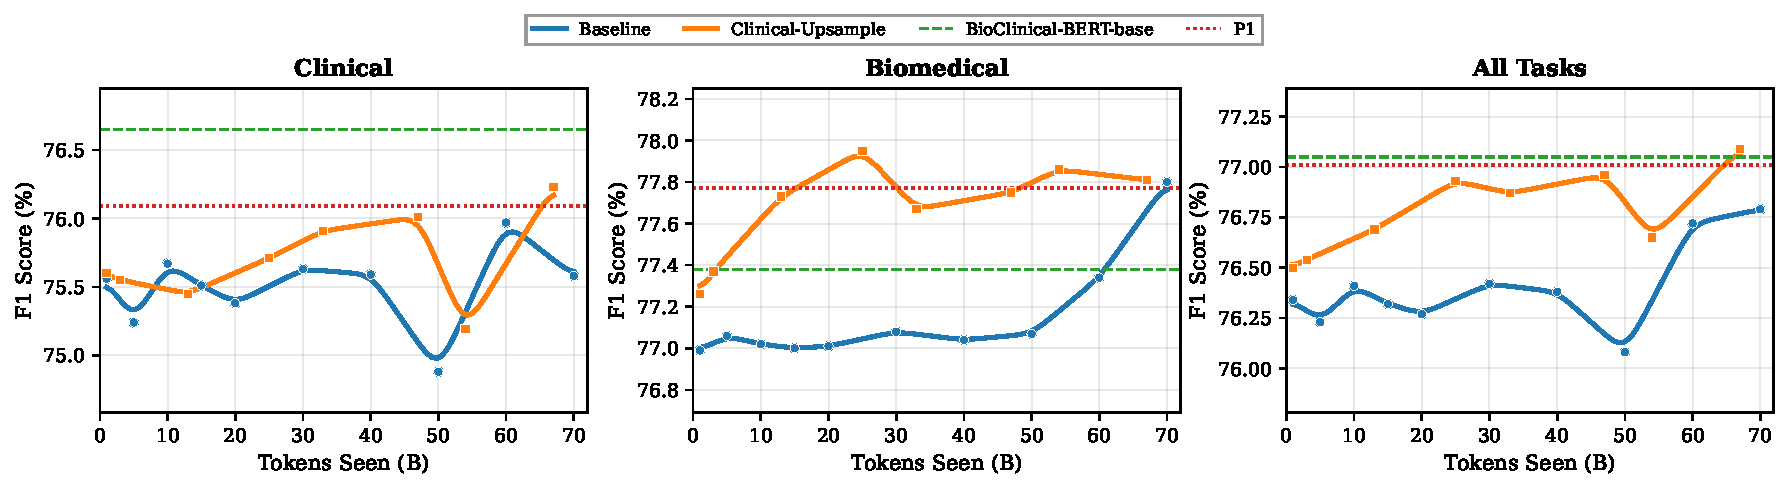
\includegraphics[width=\columnwidth]{sources/part_1/chapter2/imgs/curve_triple.pdf}
\caption{\textbf{Encoder training curves} on clinical, biomedical, and combined benchmarks. Our clinical-upsample recipe (orange) reaches higher performance faster on clinical tasks. At 67B tokens, we match BioClinical-ModernBERT (green dashed) which required 169B tokens and 20 clinical datasets.}
\label{fig:encoder-curves}
\end{figure}


\section{Discussion}
\label{sec:discussion}

The core advantage of paragraph-level annotation lies in its ability to identify valuable content that would be missed by document-level approaches. Clinical case descriptions, for instance, often appear in isolated sections of broader scientific articles. By operating at the paragraph level, we extracted 2 million clinical case paragraphs from PMC Open Access. This content is otherwise difficult to obtain at scale due to privacy restrictions on hospital records.

For decoders, our results reveal clear task-specific benefits from different enrichment strategies. Educational filtering improves knowledge-intensive QA tasks, clinical upsampling enhances clinical reasoning benchmarks, and the combination of both yields the best overall performance with faster convergence. The successful French adaptation through targeted upsampling further demonstrates that this framework generalizes beyond English. However, aggressive clinical upsampling can reduce performance on general biomedical tasks like College Biology, suggesting a trade-off between specialization and breadth.

For encoders, the decay phase experiments reveal that different paragraph types benefit different downstream tasks: Study paragraphs improve NER performance, Clinical Case paragraphs improve social history extraction, and Review paragraphs excel on relation extraction. The distinct task-specific strengths of each decay variant suggest a promising direction: model merging or checkpoint averaging could combine the benefits of specialized training runs without requiring additional compute. Rather than training general-purpose models on massive undifferentiated corpora, these findings support a more modular approach where data composition is tailored to downstream requirements.


\section{The Risks of Neural Quality Filtering}%
\footnote{This section is based on our contribution to \citet{godey_gaperon_2026}.}
\label{sec:biahs}

The results above show that selecting content by type and educational quality can improve pretraining efficiency. A natural next step is to apply neural quality classifiers, as done by FineWeb-Edu~\citep{penedo2024fineweb} and DCLM~\citep{li2024datacomp}, to filter pretraining data more aggressively. However, this raises a question: do these classifiers treat all content equally, or do they have blind spots?

To investigate this, we designed Benchmark-In-A-HayStack (BiaHS), an experiment to test how different text-quality classifiers rank benchmark-like content within a large web corpus. We sampled 35 benchmark instances from three datasets: 15 samples from MMLU (3 samples each from anatomy, computer security, high school geography, moral scenarios, and college physics), 10 from GSM8K~\citep{cobbe2021gsm8k}, and 10 from GPQA~\citep{rein2023gpqa}. Each benchmark sample was formatted as a standalone document containing the question, answer choices, and reference solution. These 35 benchmark documents were inserted as independent entries into a corpus of 99,965 documents sampled from FineWeb, yielding a final evaluation set of 100,000 documents where benchmarks constituted 0.035\% of the total.

We scored all documents using four quality classifiers: DCLM (FastText-based, used to filter OLMo~2 training data), Textbook (FastText-based, used to filter OLMo~1 training data), FineWeb-Edu (transformer-based), and the GAPeron classifier (transformer-based). Each classifier produced a full ranking of all documents based on their predicted quality score.

\begin{figure}[t]
\centering
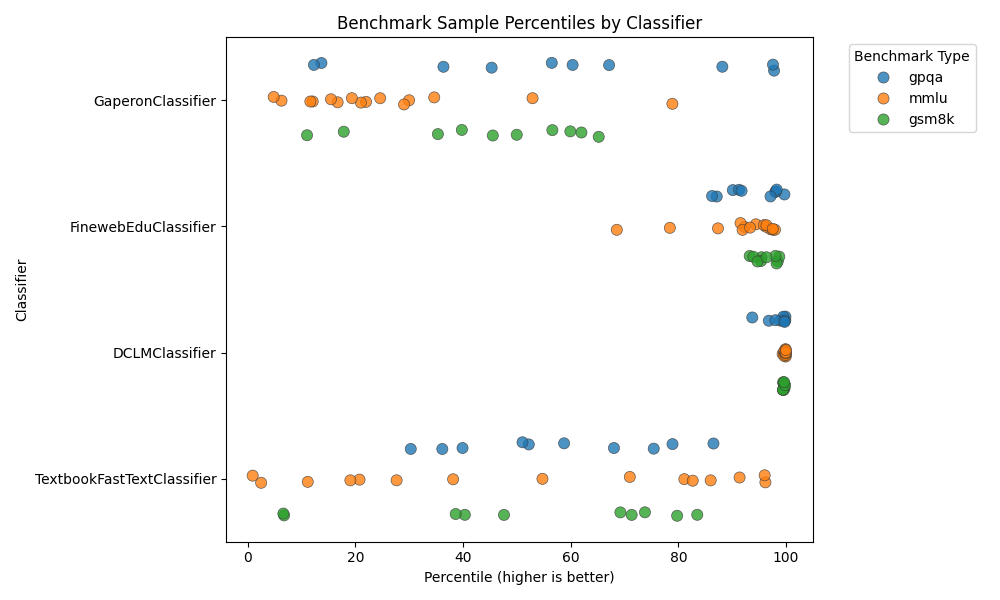
\includegraphics[width=\columnwidth]{sources/part_1/chapter2/imgs/biahs_percentiles.png}
\caption{\textbf{BiaHS: Benchmark-In-A-HayStack results.} Percentile rank of 35 benchmark samples (MMLU, GSM8K, GPQA) within 100K FineWeb documents, as scored by four quality classifiers. DCLM ranks all benchmark samples in the top-5 percentiles.}
\label{fig:biahs}
\end{figure}

The results reveal a striking pattern. The DCLM classifier ranks all MMLU and GSM8K samples in the top-5 percentiles. If only the top 5\% of documents are selected through filtering, the probability of encountering a benchmark sample in a training batch increases by a factor of approximately 20. The FineWeb-Edu classifier also ranks benchmark samples consistently higher, likely because its annotation prompt explicitly asks for documents with high educational value, which naturally favors exam-style items and step-by-step solutions.

The DCLM classifier pushes benchmark samples even higher and more consistently. Its FastText model is trained to separate synthetically generated instructions from high-scoring Reddit posts, from general web text. This training objective naturally favors solved Q\&A structures with a short question, a direct answer, and brief reasoning, which aligns with the format of common benchmark datasets.

In contrast, the GAPeron classifier does not significantly push benchmark samples. It was trained on annotations focused on general content quality across multiple dimensions: accuracy, clarity, coherence, grammar, depth of information, and overall usefulness. This broader framing does not specifically reward the structured question-answer format typical of benchmark samples.

\paragraph{Implications.} This experiment suggests that the way quality classifiers are trained can strongly influence contamination risks. As neural quality filtering becomes a standard step in data curation, these design choices deserve closer examination. For the Biomed-Enriched work presented earlier in this chapter, we rely on content-type classification and educational quality scoring rather than general quality filtering, which avoids this particular risk.


\section{Limitations}

Our decoder experiments used 7B parameter models. Larger models may respond differently to data curation choices. The two-stage annotation pipeline relies on XLM-RoBERTa-base, which may have limited capacity for nuanced paragraph classification. Our clinical case paragraphs come from published case reports, which may differ stylistically from actual hospital records. The educational quality scores are neural heuristics rather than gold-standard pedagogical assessments.

For the BiaHS experiment, the evaluation was conducted on a relatively small number of benchmark samples (35) inserted into a single web corpus (FineWeb). While the results are directionally clear, a larger-scale study across multiple corpora would strengthen the conclusions.


\section*{Conclusion}

Two findings emerge from this chapter. First, paragraph-level annotation reveals that scientific articles are far more heterogeneous than their metadata suggests: 91.6\% mix content types, and educational quality varies by 2.6 points within a single article. Selecting the right paragraphs allows matching full-corpus performance with a third of the tokens, and extracting 2 million clinical case paragraphs provides public clinical text without data use agreements.

Second, not all filtering is created equal. Neural quality classifiers trained on instructional or educational content can amplify benchmark contamination by a factor of 20, effectively turning a data curation step into a memorization accelerator. Content-type classification, by contrast, selects for relevance rather than format, and does not carry this risk.

\vspace{2em}

We now have both a general biomedical corpus (\textit{biomed-fr}, \Cref{chap:collecting}) and a method for selecting the most relevant paragraphs within it. The next chapter addresses how to combine these resources into a curated training mix, and how quality signals can be used at scale to build a better corpus for pretraining ModernCamemBERT-bio.


\chapter{Which Quality Signals Matter?}
\label{chap:mcbio}
% This chapter is based on the corpus contribution of:
%   Rian Touchent, Éric de la Clergerie.
%   ModernCamemBERT-bio: un encodeur biomédical et clinique français à contexte long.
%   TALN 2026.
%
% Source: publications/TALN2026_MB-BIO/
% This chapter covers only the corpus (biomed-fr-v2). The pretraining and evaluation
% are presented in \Cref{chap:objectives}.

\section{Introduction}

Here is one passage as it came out of an ISTEX PDF:

\begin{quote}\small\ttfamily
\dots{} vise \textasciitilde{} remonter l\&apos;organe prolab6 (correction de la pt6se) et h le soutenir dans sa position id6ale plus qu\&apos;/\textasciitilde{} le fixer (fixation). Ce sout\textasciitilde{}nement est assur6 par le renforcement du p6rin6e grace aux tissus naturels que l\&apos;on r6pare (rapphie) ou que l\&apos;on consolide avec du mat6riel local (plastie, ligamentopexie)\dots{}
\end{quote}

\noindent And here is what it should read:

\begin{quote}\small
\dots{} la chirurgie vise à remonter l'organe prolapsé (correction de la ptose) et à le soutenir dans sa position idéale plus qu'à le fixer (fixation). Ce soutien est assuré par le renforcement du périnée grâce aux tissus naturels que l'on répare (raphie) ou que l'on consolide avec du matériel local (plastie, ligamentopexie)\dots{}
\end{quote}

\noindent OCR had read every \emph{é} as a \emph{6}, apostrophes came as \texttt{l\&apos;}, and tildes had drifted into the middle of words. Multiply this by the hundreds of thousands of similar PDFs in HAL and ISTEX, and assembling a 10-billion-token biomedical training mixture stops being a collection problem and becomes a repair problem.

\Cref{chap:collecting} introduced \textit{biomed-fr}, a 413-million-word public French biomedical corpus. \Cref{chap:quality} showed that paragraph-level annotation by a large language model can identify content types and educational quality more precisely than document-level filters, and that neural quality classifiers carry contamination risks. This chapter applies these lessons at scale. We assemble \textit{biomed-fr-v2}, a 10-billion-token mixture from six French sources, and ask which quality signals actually improve downstream performance once the dust settles. The corpus is the training data for ModernCamemBERT-bio, presented in \Cref{chap:objectives}.

The contributions of this chapter are: (1) a multi-source French biomedical corpus 25 times larger than \textit{biomed-fr}, including a curation pipeline that handles the OCR artifacts, boilerplate, and structural noise of HAL and ISTEX; (2) an LLM-based annotation of 2.16 million paragraphs along four quality signals and nine content types; (3) ablation studies that quantify the effect of each signal and each type on downstream performance, with one notable surprise: writing-quality and terminological-precision filters \emph{degrade} performance.


\section{Sources}
\label{sec:corpus-sources}

We assemble \textit{biomed-fr-v2} from six complementary French-language sources. HAL, ISTEX, and FineWiki-bio cover scientific biomedical literature. EMEA contributes drug package inserts. E3C contributes clinical case reports. Synthetic textbooks generated from medical ontologies complete the mixture with the vocabulary of French administrative nomenclatures. The final composition is summarized in \Cref{tab:mcbio-corpus}.

\begin{itemize}
\item \textbf{HAL.} Medical theses, research articles, and reports deposited on the HAL open archive, filtered to the biomedicine section.
\item \textbf{ISTEX.} French scientific articles from the ISTEX corpus, filtered to biology and medicine.
\item \textbf{FineWiki-bio.} Biomedical subset of FineWiki, the Wikipedia counterpart to FineWeb~\citep{penedo2024fineweb}, restricted to French and filtered for the biomedical domain.
\item \textbf{EMEA}~\citep{neveol14quaero}. Drug package inserts published in French by the European Medicines Agency.
\item \textbf{E3C}~\citep{magnini_e3c_2021}. Multilingual clinical corpus (layer 3, French partition), composed of clinical cases extracted from medical journals and theses.
\item \textbf{Synthetic ontology textbooks.} Educational text generated from three French medical ontologies published by the Agence du Numérique en Santé in RDF/OWL format: CIM-10 (diagnoses, 19{,}161 codes), CCAM (procedures, 38{,}191 codes), and ATC (medications, 6{,}950 codes). Random walks through the ontology graph (1.3 million walks total) traverse hierarchical relations and, for CIM-10, causal and exclusion relations. A large language model (Qwen3-235B-A22B-Instruct) reformulates each walk into a paragraph of medical prose while preserving the original codes and relations. The full pipeline is described in \Cref{chap:ontobook}.
\end{itemize}

HAL and ISTEX are distributed in heterogeneous formats: some documents come with structured XML, others only as PDFs, sometimes scans of printed material. For documents without clean XML, we apply the extraction and cleaning pipeline described in \Cref{sec:corpus-pipeline}. FineWiki-bio, EMEA, E3C, and the synthetic textbooks are already of high quality and are integrated directly into the final mixture, bypassing this pipeline.


\section{Curation Pipeline}
\label{sec:corpus-pipeline}

A portion of HAL and ISTEX documents come with clean XML and proceed directly to annotation. The other portion is available only as PDFs, sometimes scans of printed material (particularly for articles published before the 1990s). Once converted to text, these PDFs contain OCR artifacts (incorrect ligatures, character substitutions, fragmented words), bibliographic references, repeated headers, and irrelevant content. We therefore apply an LLM-based extraction and cleaning pipeline, described below. The other sources (FineWiki-bio, EMEA, E3C, synthetic textbooks) are already clean and bypass this pipeline entirely.

\paragraph{Extraction and cleaning.} Each document is split into segments of approximately 5{,}000 tokens at paragraph boundaries. A large language model (Qwen3-Next-80B-A3B-Instruct) receives each segment and produces structured JSON output containing semantically complete passages, with references, metadata, headers, and captions removed, and OCR errors corrected (ligatures, encoding). Extracted passages must contain between 30 and 600 words and at least 60\% alphabetic characters. We then apply Jaccard-similarity deduplication (threshold 0.80, sliding window of 5 passages), followed by the FineWeb-2 filter chain for French: encoding correction, repetition filters, and Gopher and FineWeb quality filters.

\paragraph{Fidelity verification.} To ensure the LLM does not introduce content absent from the source, we measure character-level overlap between each extracted passage and its source document on 300 ISTEX passages (after typographic normalization). 94.4\% of passages have $\geq 90$\% overlap and 84.1\% have $\geq 99$\% overlap; the median rate of words absent from the source is zero (mean: 3.4\%). Manual inspection of edge cases shows that divergences come from OCR corrections (such as the surgical passage shown at the start of this chapter) or from converting tables into prose. The opposite case is also common: a clean 1{,}143-character passage on cancer-related depression is extracted with 100\% character overlap and no additional words introduced. These two cases bracket the typical behavior of the pipeline: it cleans aggressively when the source is corrupted by OCR, and copies verbatim when the source is already clean.

\paragraph{LLM quality annotation.} The same LLM annotates each passage along four quality signals scored from 1 to 10: educational value (\texttt{edu}, mean 6.5), content richness (\texttt{cont}, 6.8), writing quality (\texttt{writ}, 7.6), and terminological precision (\texttt{term}, 7.6). The codes in parentheses are the abbreviations used in ablation tables. A content type is also assigned among nine categories: \texttt{research\_findings} (526k passages), \texttt{medical\_knowledge} (388k), \texttt{clinical\_guidance} (218k), \texttt{research\_methodology}, \texttt{drug\_information}, \texttt{background\_review}, \texttt{policy\_administrative}, \texttt{patient\_case} (36k), and \texttt{other}. In total, 2.16 million passages are annotated.


\section{Content-Type Ablation}

We measure the effect of each content type by ablation: we remove one type and compare against the full corpus on three evaluation tasks (DiaMed, FrACCO-30, and EMEA, 9 seeds). \Cref{tab:mcbio-content-type} shows that removing \texttt{drug\_information} \emph{improves} performance by $+0.67$pp, while removing \texttt{medical\_knowledge} degrades it by $-0.13$pp. A random control (removing the same amount of text at random) gives $+0.04$pp, confirming that the effect is specific to the content type.

\begin{table}[t]
\centering
\small
\setlength{\tabcolsep}{8pt}
\begin{tabular}{lcc}
\toprule
\textbf{Type removed} & \textbf{Avg $F_1$} & $\boldsymbol{\Delta}$ \\
\midrule
\rowcolor{ThesisTableSep}
\multicolumn{3}{c}{\rule{0pt}{10pt}\textbf{Removal helps}} \\[1pt]
\texttt{drug\_information} & 64.35 & $+$0.67pp \\
\texttt{research\_findings} & 64.24 & $+$0.56pp \\
\texttt{policy\_administrative} & 64.07 & $+$0.39pp \\
\midrule
\rowcolor{ThesisTableSep}
\multicolumn{3}{c}{\rule{0pt}{10pt}\textbf{Controls}} \\[1pt]
Random (same volume) & 63.72 & $+$0.04pp \\
Full corpus (reference) & 63.68 & ref. \\
\midrule
\rowcolor{ThesisTableSep}
\multicolumn{3}{c}{\rule{0pt}{10pt}\textbf{Removal hurts}} \\[1pt]
\texttt{medical\_knowledge} & 63.55 & $-$0.13pp \\
\texttt{research\_methodology} & 63.51 & $-$0.17pp \\
\bottomrule
\end{tabular}
\caption{\textbf{Content-type ablation.} We remove one type and measure $\Delta$ relative to the full corpus.}
\label{tab:mcbio-content-type}
\end{table}

We exclude \texttt{drug\_information} from the final corpus (redundant with the EMEA source already included separately) and \texttt{other}. Paragraphs shorter than 50 tokens are also excluded.


\section{Quality Filtering and Upsampling}
\label{sec:upsampling}

We then test the effect of thresholding on the quality signals (\Cref{tab:mcbio-quality-signals}). Joint filtering with \texttt{edu}$\geq 7$ and \texttt{cont}$\geq 7$ produces a $+0.48$pp gain; a stricter threshold (\texttt{edu}$\geq 8$ and \texttt{cont}$\geq 8$) reaches $+0.55$pp. By contrast, the writing-quality and terminological-precision signals \emph{degrade} performance when used as filters ($-0.26$ and $-0.33$pp). This degradation likely comes from the fact that these filters eliminate informal but informative clinical documents, such as case notes and lightly edited reports.

\begin{table}[t]
\centering
\small
\setlength{\tabcolsep}{8pt}
\begin{tabular}{lcc}
\toprule
\textbf{Filter} & \textbf{Avg $F_1$} & $\boldsymbol{\Delta}$ \\
\midrule
\rowcolor{ThesisTableSep}
\multicolumn{3}{c}{\rule{0pt}{10pt}\textbf{Helpful filters}} \\[1pt]
\texttt{edu}$\geq 8$ AND \texttt{cont}$\geq 8$ & \bfseries 59.37 & $+$0.55pp \\
\textbf{\texttt{edu}$\geq 7$ AND \texttt{cont}$\geq 7$} & \underline{59.30} & \textbf{$+$0.48pp} \\
\texttt{edu}$\geq 6$ AND \texttt{cont}$\geq 6$ & 58.95 & $+$0.13pp \\
\midrule
No filter (reference) & 58.82 & ref. \\
\midrule
\rowcolor{ThesisTableSep}
\multicolumn{3}{c}{\rule{0pt}{10pt}\textbf{Harmful filters}} \\[1pt]
\texttt{term}$\geq 7$ & 58.57 & $-$0.26pp \\
\texttt{writ}$\geq 7$ & 58.49 & $-$0.33pp \\
\bottomrule
\end{tabular}
\caption{\textbf{Quality-signal ablation.} Educational value and content richness improve performance; writing quality and terminological precision degrade it.}
\label{tab:mcbio-quality-signals}
\end{table}

Rather than applying a strict filter, we adopt a quality-weighted upsampling inspired by FineWeb~\citep{penedo2024fineweb}. Each article receives a quality ratio, defined as the proportion of its paragraphs satisfying \texttt{edu}$\geq 7$ AND \texttt{cont}$\geq 7$. Articles are then upsampled in proportion to this ratio (\Cref{tab:mcbio-upsampling}). Articles with 0\% high-quality paragraphs are excluded from the final corpus.

\begin{table}[t]
\centering
\small
\setlength{\tabcolsep}{12pt}
\begin{tabular}{lr}
\toprule
\textbf{Ratio of \texttt{edu}$\geq 7$ AND \texttt{cont}$\geq 7$ paragraphs} & \textbf{Coefficient} \\
\midrule
0\% & excluded \\
1--25\% & 4.3$\times$ \\
26--50\% & 8.5$\times$ \\
51--75\% & 12.8$\times$ \\
76--99\% & 21.3$\times$ \\
100\% & 34.1$\times$ \\
\bottomrule
\end{tabular}
\caption{\textbf{Upsampling coefficients} per article-quality bucket.}
\label{tab:mcbio-upsampling}
\end{table}


\section{Final Composition}

The final training mixture, after cleaning and quality-weighted upsampling, contains 10 billion tokens (\Cref{tab:mcbio-corpus}). These 10 billion include the repetitions induced by upsampling (coefficients ranging from 4.3$\times$ to 34.1$\times$ depending on quality, see \Cref{sec:upsampling}); the underlying unique content is more limited. HAL and ISTEX articles (passed through the pipeline of \Cref{sec:corpus-pipeline}) and FineWiki-bio (integrated as-is) are grouped under ``curated biomedical articles.'' The three other sources (EMEA, E3C, synthetic textbooks) are also integrated as-is.

\begin{table}[t]
\centering
\small
\setlength{\tabcolsep}{10pt}
\begin{tabular}{lrrl}
\toprule
\textbf{Source} & \textbf{Tokens} & \textbf{\%} & \textbf{Content} \\
\midrule
Curated biomedical articles & 7B & 70\% & HAL + ISTEX + FineWiki-bio \\
Synthetic ontology textbooks & 2B & 20\% & CIM-10, CCAM, ATC \\
EMEA (drug inserts) & 600M & 6\% & Pharmacology \\
E3C (clinical sentences) & 400M & 4\% & Patient cases \\
\midrule
\textbf{Total} & \textbf{10B} & \textbf{100\%} & \\
\bottomrule
\end{tabular}
\caption{\textbf{Composition of the \textit{biomed-fr-v2} training mixture} after quality-weighted upsampling.}
\label{tab:mcbio-corpus}
\end{table}


\section*{Conclusion}

Two findings emerge from the ablations. First, not all content types contribute equally: removing drug information actually improves downstream performance, while removing medical knowledge degrades it. Second, not all quality signals work as filters: educational value and content richness help, but writing-quality and terminological-precision filters \emph{hurt} performance, likely because they remove the informal but informative clinical documents that ultimately matter most. The lesson, perhaps, is that curation should be guided by what is being said, not by how well it is written.

\vspace{2em}

The corpus is now ready. The next two chapters use it to train French biomedical encoders. \Cref{chap:encoders} starts with the simplest recipe (continual pretraining with MLM on \textit{biomed-fr}) and shows that even a modest public corpus produces a competitive model. \Cref{chap:objectives} returns to \textit{biomed-fr-v2} with a more ambitious recipe: a temporary detour through causal language modeling that, somewhat unexpectedly, leaves a permanent imprint on the encoder.

